% Activate the following line by filling in the right side. If for example the name of the root file is Main.tex, write
% "...root = Main.tex" if the chapter file is in the same directory, and "...root = ../Main.tex" if the chapter is in a subdirectory.
 
%!TEX root =  

\chapter{Project Directive}
\minitoc

\section{Purpose}
This document describes the mandate, background, resources available and organizational structure of the project �Privacy Advisor�, henceforth referred to as �the project�.

\section{Mandate}
The purpose of this project is to implement the key functionality of a privacy agent as described in Nyre and T�ndel (2010), that provides users with advice in making Internet privacy decision. 

\subsection{Background}
This project is a part of a larger research project at SINTEF ICT that studies approaches to handling Internet privacy related issues. The underlying idea is that while users are often concerned about the way various websites and services handle private information about them, obtaining information about this is very costly as privacy policies tend to be very long documents formulated in an inaccessible language. This has led to the idea that Internet privacy can be handled by machine learning techniques, where a particular decision is based on the user�s past behavior and the behavior of similar users.

Nyre and T�ndel has then proposed a �Privacy Agent� structure that uses the case based reasoning (CBR) method for giving privacy advice. CBR is in many ways similar to the way human experts reason about problems, and is usually described as a process in four stages (here related to the privacy decision problem):
\begin{itemize}
\item Retrieve: 
Given a new site, the agent will retrieve from its knowledge base, the set of cases deemed the most similar to the one at hand. This means, that if presented with the site Facebook, for instance, the agent finds Twitter, Google and LinkedIn to be the sites that have the most similar policy to Facebook.
\item Reuse: 
Look at the decisions made about the cases that were found and adapt this decision to the problem at hand. In this case, the agent needs to see if there are strong enough indications toward a particular behavior with respect to the type of site that is at hand. If for instance, the user has accepted the policies of all the similar sites found, he is also likely to accept that of Facebook.
\item Revise: 
Once a conclusion is reached, it is presented to the user (along with the background for why it is reached). The user may then choose to accept the conclusion, or to overrule it, providing the system with directions as to why it was wrong. This may in turn cause the agent to update its parameters accordingly. 
\item Retain: Finally, the new case is stored to the database along with the user�s decision as a reference for the next time the same site is opened, and as a case to employ when evaluating new sites.
\end{itemize}

Nyre and T�ndel also describes this local CBR approach to be complemented by a community database where the same information is stored, allowing for a second lookup that uses a collaborative filtering, that is, making a decision based on the behavior of similar users.

\section{Objectives}
This project identifies three key objective, arranged by order of importance:
Implementing a testing framework of CBR based privacy agent that is able to make privacy decisions based on previous user behavior.
Implement the community system/collaborative filtering part of the agent.
Extend the system to other standards for machine readable privacy policies.
Implement the system as a browser plugin. This is considered least important, and is contingent on the success of early testing. It is also given a low priority given the relative small portion of major websites that implement P3P.


\section{Resources and Duration}
The system in its complete form is to be demonstrated on November 24 2011. For the project period, a total of 25 hours per week per project member is planned. With seven group members and a project spanning 13 weeks, this adds up to approximately 2300 hours.

\section{Organization}
Project management is based a standard model where the customer takes on the role of \emph{project owner} or simply "owner". The project owner is the actual stakeholder and initiator of the project, and responsible for all executive decisions in the project. The \emph{project group} or \emph{team} is responsible for delivering the product in accordance with the wishes of the customer as defined by the \emph{requirements specification} document. Two project management roles are designated, one is responsible for administrative decisions, hereunder planning, reporting, calling meetings, customer contact and so forth. The second management role is that of chief system architect, who has the responsibility and final word in all technical decisions.

\begin{figure}[htbp]
\begin{center}
\caption{Project Organization}
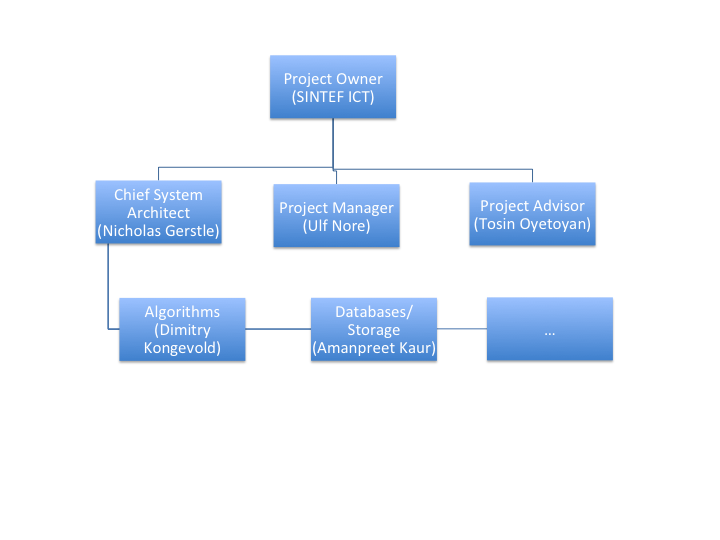
\includegraphics[width = 1.0\textwidth]{ProjectDirective/Org.png}
\label{Organization}
\end{center}
\end{figure}



The project group organization is based on the modules of the system that is being implemented, this is often referred to as a \emph{functional} structure or organization. One group member is responsible for developing one particular feature. This organization is shown in Table~\ref{orgTable}. In addition to this internal functional organization, two project managers are appointed, one having responsibilities for administrative decisions and reporting and one with responsible for technical decisions.

 

\begin{table}[htdp]
\caption{Responsibilities}
\begin{center}
\begin{tabularx}{\textwidth}{| X | X | X |}
\hline
\textbf{Role} & \textbf{Description} &\textbf{Responsible} \\
\hline
Administrative 	&  Customer relations  & Ulf Nore \\
			& Requirement specification & \\
			& Requirement specification & \\
			& Planning documents & \\
			& Meeting minutiae & \\
			& Project report & \\	
\hline					
Software design and Architecture   	&  UML modeling.	 	& Nicholas Gerstle \\ 
						      	& Design report.		& \\
							& User documentation.	& \\
							& Technical Decisions.	& \\
\hline
Data Storage/Databases	& Flat file data storage system. 	& Amanpreet Kaur \\
					& Database systems	.			& \\
\hline
CBR - Algorithms and Data structures 	& Data structures for storing privacy policy information.	& Dimitry Kongevold,\\
								& Define and implement similarity metrics.			& Neshahavan Karunakaran \\
								& Retrieval and learning algorithms. &	\\
								& Parameter storage. & \\
\hline
Testing and Evaluation 	& Design test cases. & Henrik Knutsen \\
					& Criteria/methodology for model testing. & \\
\hline
GUI & Implement a simple GUI for testing model framework. & Ulf Nore \\
\hline
Version control & Set up and maintain code repository. & Einar Afiouni \\
\hline
XML/P3P Parser & Implement P3P parser that produces inputs to CBR & Einar Afiouni \\
\hline
Version control & Set up and maintain code repository. & Einar Afiouni \\								 	
\hline
\end{tabularx}
\end{center}
\label{orgTable}
\end{table}%



\section{Planning}
A project plan has been developed for the purpose of communicating expectations and progress within the group and to the customer and the advisor. The plan also serves as an aid in identifying problems and project management. For the software development process, a hybrid waterfall model has been chosen.


\section{Limitations and Scope}
The primary focus of this project is on developing a framework that allows for testing the CBR privacy agent framework. This entails building a module for parsing policy documents in XML format, a data structure for holding policy information in memory (henceforth �policy objects�), a set of exchangeable distance metric that compares policy objects, a generic retrieval algorithm (such as k Nearest Neighbors) that works with any distance metric and methods to store and update a knowledge base. Being a part of an ongoing research project, reusability and modularity are important success factors for in evaluating the project. This means that it should for instance be simple to swap P3P with some other privacy policy standard, that different distance metrics should be applicable, new metrics could easily be implemented and so forth.
